\points{3a} \textbf{Implementing the Exact Score Matching}

To implement the Exact Score Matching objective, you are required to complete the following functions within the provided code in the \texttt{score\_matching\_utils.py} and \texttt{score\_matching.py} files:

\begin{itemize}
    \item \texttt{log\_p\_theta} 
    \item \texttt{compute\_score} 
    \item \texttt{compute\_divergence}
    \item \texttt{compute\_l2norm\_squared}
    \item \texttt{score\_matching\_objective}
\end{itemize}

Run the score matching experiment using the following command:
\begin{lstlisting}[language=bash]
    python run_score_matching.py
\end{lstlisting}

Your implementation should generate the following results:
\begin{figure}[H]
    \centering
    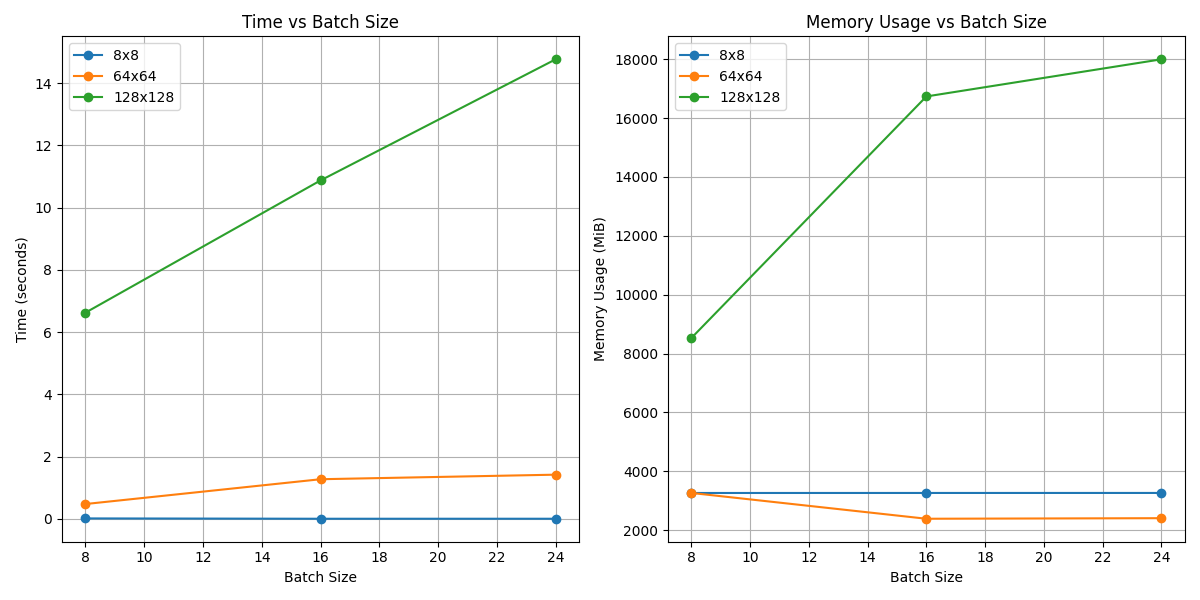
\includegraphics[width=0.8\textwidth]{./figures/score_matching_results}
    \caption{Score Matching Output Graphs}
\end{figure}